\documentclass[a4paper,12pt]{article}
\parindent 0pt
\parskip 1mm
\usepackage{amsmath}
\usepackage[dvips]{epsfig}

\begin{document}

\begin{center}

{\Large\bf CN 530 - Neural and Computational Models of Vision}

\bigskip

{\large\bf Assignment \# 10}
\smallskip

{\large\bf John Joseph}
\end{center}

\bigskip
{\bf Simulation Assignment 1}
\bigskip

{\bf Item 1 Part a}
\bigskip

We are asked to solve for the equilibrium solution of following differential equation:

\begin{equation}
\frac{dx_i}{dt} = -Ax_i+(B-x_i)I_i-x_i \sum_{k \neq i}I_k
\end{equation}

Setting the equation equal to 0, we see that

\begin{equation}
0 = -Ax_i+(B-x_i)I_i-x_i \sum_{k \neq i}I_k
\end{equation}

\begin{equation}
0 = BI_i-x_i(A+I_i+\sum_{k \neq i}I_k)
\end{equation}

\begin{equation}
x_i = \frac{BI_i}{A+I_i+\sum_{k\neq i}I_k}
\end{equation}

This is the equilibrium solution of $x_i$, the response of node $i$ to a given input $I_i$. Note that $x_i$ is bounded between 0 and $B$. 

\vspace{2mm}

This equation, when logarithmically plotted, demonstrates the shift property useful in preserving signals in varying luminances. We can denote the background intensity $\sum_{k\neq i}I_k$ as $L_j$, the luminance. In logarithmic scale, the linear shift $S$ is equal to 

\begin{equation}
S=log(A+L_2)-log(A+L_1)
\end{equation}

See the plot below:

\vfil\eject

\begin{center}
  \begin{figure}[h!]
    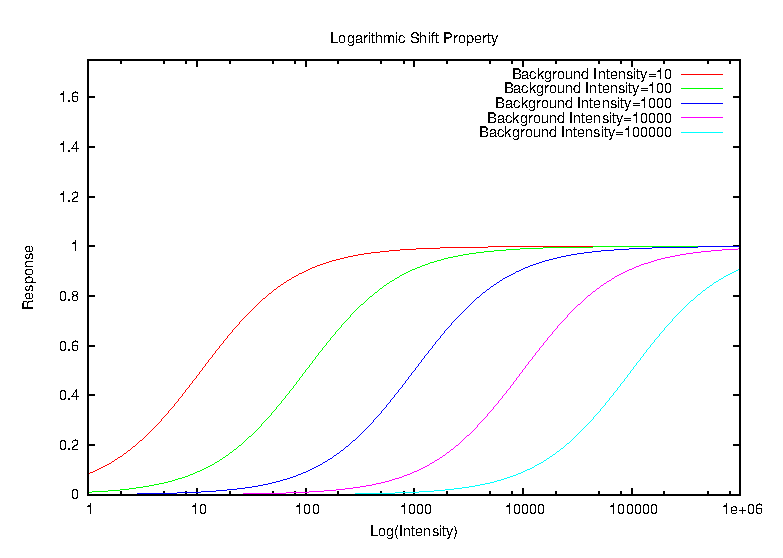
\epsfig{file=figures/logShift.eps,width=15cm,height=11cm}
    \caption{\label{pict1}Equilibrium Response, A=1.0, B=1.0}
  \end{figure}
\end{center}

We see the preservation of our response in varying background intensities, which is a very useful property that maintains visual response in different environments. The maximum response is controlled by $B$, but notice that relatively low responses are sent to 0. 

\bigskip
{\bf Item 1 Part b}
\bigskip

We now examine the differential equation

\begin{equation}
\frac{dx_i}{dt} = -Ax_i+(B-x_i)I_i-(x_i+C) \sum_{k \neq i}I_k
\end{equation}

at equilibrium. 

\vfil\eject

Using the same method as before, we find the equilibrium response to be

\begin{equation}
x_i =  \frac{BI_i-C\sum_{k\neq i}I_k}{A+I_i+\sum_{k\neq i}I_k}
\end{equation}

The $C$ term changes our response bound to range within $-C$ and $B$. When plotting this response we see similar results. 

\begin{center}
  \begin{figure}[h!]
    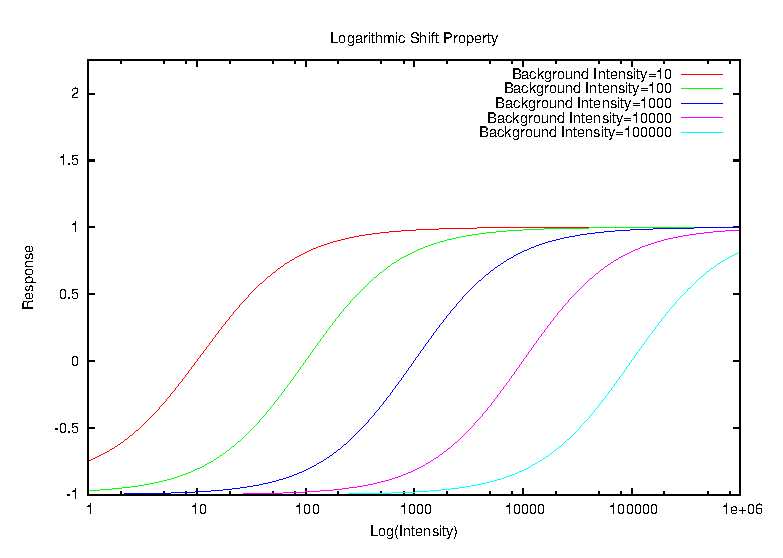
\epsfig{file=figures/logShift_C.eps,width=15cm,height=11cm}
    \caption{\label{pict1}Equilibrium Response, A=1.0, B=1.0, C=1.0}
  \end{figure}
\end{center}

Notice that we've doubled our effective range by including the $C$ term. This property allows for pattern preservation at higher intensities, reducing the saturation that may have occured otherwise. If this is unclear, consider the following plot:

\begin{center}
  \begin{figure}[h!]
    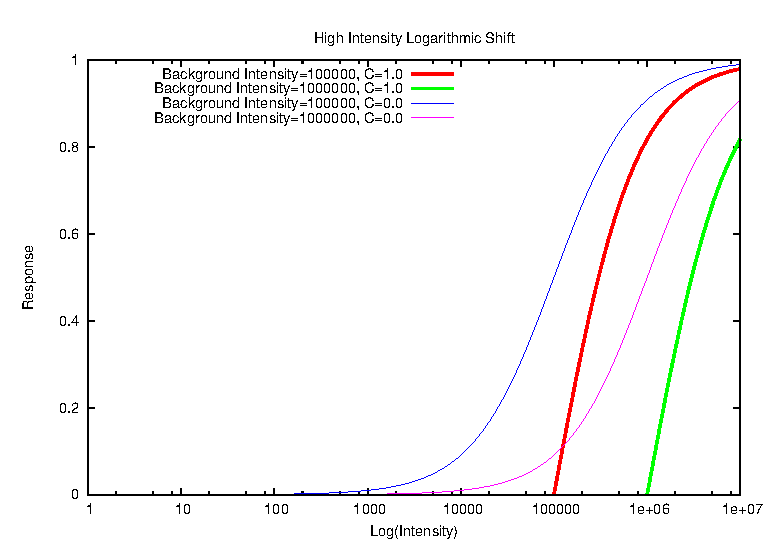
\epsfig{file=figures/highIntensity.eps,width=15cm,height=7cm}
    \caption{\label{pict1}Equilibrium Response for High Intensities}
  \end{figure}
\end{center}

Here the thicker lines represent the new network equation; note that we've effectively doubled the difference in response between these two background intensities. Below is a plot of this difference, making it clear that we get a much lower level of saturation when we include the $C$ term and increase our range of response. 

\begin{center}
  \begin{figure}[h!]
    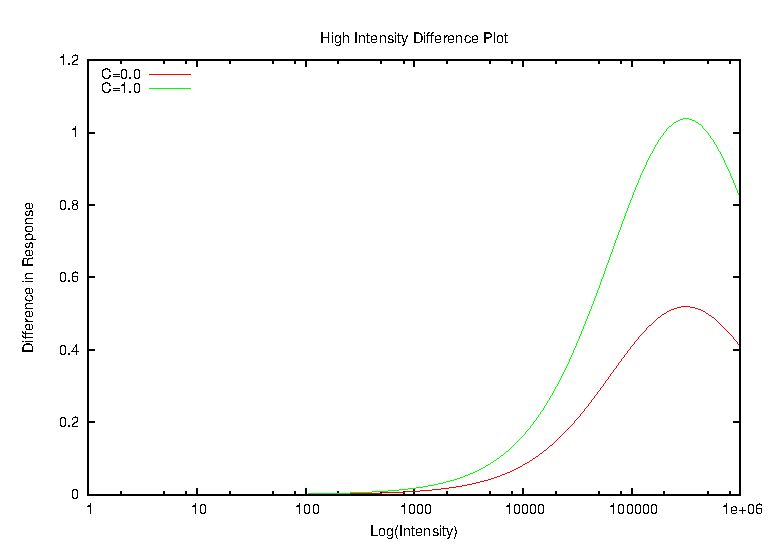
\epsfig{file=figures/diff.eps,width=15cm,height=7cm}
    \caption{\label{pict1}Difference In Equilibrium Response between L=1e5 and L=1e6}
  \end{figure}
\end{center}



By increasing the difference in response between different intensities we improve the ability for our network to make out individual stimuli, and in doing so prevent input from being lost due to saturation. 

\bigskip
{\bf Item 2}
\bigskip

The difference in response between nodes in the ``center'' and nodes in the ``surround'' of our input field can be demonstrated effectively using only three nodes. Consider these three in row wherein the middle node represents the center and its two neighbors are the surround. 

\vspace{2mm}

Suppose the surround intensity is valued at 0, and the center intensity is valued at 1. The responses, using equation 1a (equation 1 in this document), are as follows:

\begin{center}
  \begin{figure}[h!]
    
\epsfig{file=figures/drawing.eps,width=15cm,height=5cm}
    \caption{\label{pict1}Equilibrium Response, A=1.0, B=1.0}
  \end{figure}
\end{center}

Though this may seem trite, the only motivation I saw to use a larger network was generating an illusion of complexity. This example demonstrates a distinct contrast between center and surround. 

\vspace{2mm}

Cells compete for the same reason anything else competes. Our brains only have so much attention to give, and by competing for that attention we can identify important features in our visual field.

\vfil\eject
{\bf Item 3}
\bigskip

Looking at the patterns in Figure 1c, I can see that there are three distinct levels of Intensity coming into the nodes. Let's suppose these three values correspond to 1 for the low surround, 2 for the center, and 3 for the high surround. 

\vspace{2mm}

In a global configuration in which we normalize input based on the entire receptive field, the responses for these inputs are 0.027, 0.054, and 0.081 respectively. This means that every contrast has an increment(decrement) of 0.027. 

\vspace{2mm}

Considering the same situation with a local normalization scheme in which we normalize the inputs on the left and right separately, we'd find that the response of inputs 1 and 2 would be 0.077 and 0.015, respectively, for the graph on the left. 

\vspace{2mm}

For the graph on the right an intensity of 2 and 3 would correspond to a response of 0.08 and 0.12, respectively. This means that for the graph on the left we'd have an increment of 0.078, and for the graph on the right we'd have a decrement of 0.04. 

\vspace{2mm}

As you can see, the local normalization scheme offers greater contrast between center/surround, which is useful to us when detecting ``edges'' in our input. The local normalization would allow us to process multiple areas of contrast in our receptive field independent of one another. 

\vspace{2mm}

A disadvantage of this model, however, is that we'd potentially lose out on our ability to hone in on one feature in particular. What this amounts to is more work for our brains for (potentially) less detail in crucial situations where we may need it. 

\vspace{2mm}

In practice I would assume our receptive fields have some sort of dynamic radius over which the inputs are normalized, similar to how a camera can be focused when needed. Each form of normalization has its use. 

\end{document}
